\documentclass[
	%a4paper, % Use A4 paper size
	letterpaper, % Use US letter paper size
]{jdf}

\addbibresource{references.bib}

\author{Andrew Myers}
\email{amyers72@gatech.edu}
\title{CS 7646: Project 3 - Assess Learners}

\begin{document}
%\lsstyle

\maketitle

\begin{abstract}
	Machine learning models can be powerful tools for making predictions, but they do have limitations.
	For example, models can be overtrained and overfit on training data, leading to poorer performance on new data.
	In this report, we will analyze different machine learning models and analyze some of their tradeoffs.
\end{abstract}

\section{Introduction}
Supervised machine learning algorithms are able to analyze data to make predictions.
However, these algorithms may not perform as well as expected due to overfitting.
Overfitting occurs when the model matches the training data too closely and can't perform as well on new data.
In this report, we will analyze the performance of a Decision Tree Learner and a Random Tree Learner on a set of data.
We will analyze their performance with respect to overifitting and experiement with the number of tree leaves.
At first glance, it seems reasonable to believe that the Decision Tree learner will perform better than the Random Tree learner because it makes data-informed decisions instead of randomness.
Similarly, it makes sense that increasing the number of leaves (by decreasing the size of leaves) in either tree will perform better as it utilizes a bigger tree with more potential outcomes.
However, both of these factors also make the models more likely to overfit.
In practice, we hypothesize that Random Tree Learners can be just as effective as Decision Tree Learners.
We believe that adjusting the tree size and utilizing bagging techniques can improve the performance of the models.

\section{Methods}

Note: All experiments will use the same training data (\%60 of data set) and testing data (\%40 of data set) to train and evaluate the models.
\subsection{Experiment 1}
First, we will look at the effect the size of leaves has on the performance of the Decision Tree Learner.
To do this, we will train the decision tree model over 60\% of the data using leaf sizes between 1 and 30.
We will then use the Root Mean Squared Error (RMSE) to measure the performance of the model on the remaining 40\% of data and see if overfitting has occurred.

\subsection{Experiment 2}
Next, we will see if utilizing bagging techniques helps improve the performance and counteracts overfitting.
To achieve this, 30 models (or bags), each trained with a random subset of 60\% of the training data from Experiment 1, will have their predictions averaged to make a final prediction.\
We will still use the Decision Tree Learner and test across a range of leaf sizes to observe the amount of overfitting that is occurring.

\subsection{Experiment 3}
Finally, we will compare the Decision Tree Learner to the Random Tree Learner.
Here, we will see if the extra "knowledge" built into the Decision Tree Learner is actually beneficial or just leads to overfitting.
Once again, both models will be trained on 60\% of the data and tested on the remaining 40\%.
However, this time their performance will be measured based on their Maximum Error (ME) and the Time it takes to train the model. % // TODO finish this


\section{Discussion}

\subsection{Experiment 1}

\begin{jdffigure}
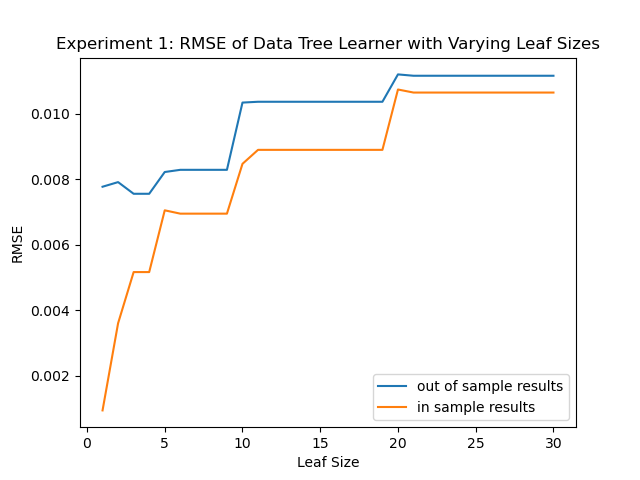
\includegraphics[height=6cm]{Figures/Figure1.png}%
\captionof{figure}{This figure shows the Root Mean Squared Error (RMSE) of Data Tree Learners trained on leaf sizes ranging from 1 and 30.}\label{fig:flowchart}%
\end{jdffigure}
First, we analyzed the performance of the Decision Tree Learner on a range of leaf sizes.
In \textbf{Figure 1}, we observe that as the leaf size increases, RMSE also increases.
This is expected as the models with fewer leaves have more potential outcomes and can better fit the data.
However, we do see signs of overfitting in \textbf{Figure 1} as leaf size decreases below 3.
Overfitting occurs because the model fits too closely to the training data and can't generalize well on new data.
It is critical to combat overfitting by not making models more complex than their training data can support (i.e. to not overtrain the models).
Otherwise, the model will start to perform worse on data that it has not seen before.
We can recognize overfitting when the in sample error decreases while the out of sample error increases.
The problem of overfitting can be combatted by averaging predictions from multiple sources, for example by bagging (explored in Experiment 2).
Alternatively, we can smooth the results of the overfit model by increasing the leaf size, which can be thought of as combining leaves together and averaging.
The data shown in \textbf{Figure 1} would suggest the optimal leaf size for the decision tree model is 3, where there are enough leaves to give precise answers, but not too many that the model is overfit.

\subsection{Experiment 2}
\begin{jdffigure}
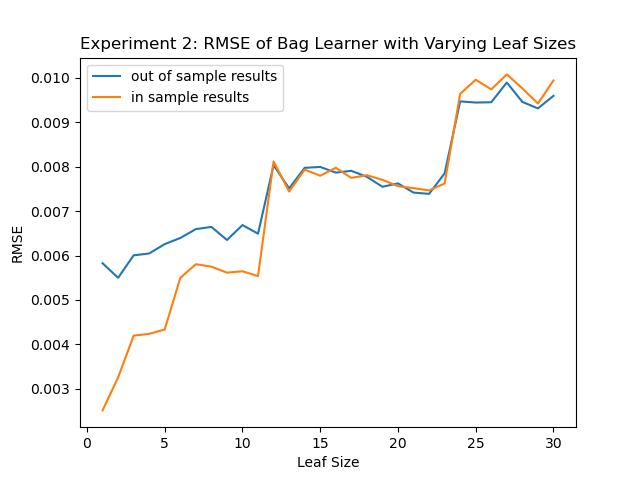
\includegraphics[height=6cm]{Figures/Figure2.png}%
\captionof{figure}{This figure shows the Root Mean Squared Error (RMSE) of a Bag Learner trained on leaf sizes ranging from 1 and 30.}\label{fig:flowchart}%
\end{jdffigure}
In the second experiment, we looked at the performance of the Decision Tree learner enhannced with bagging techniques.
By combining the results of 30 models, we canexpect to  improve the performance of the model and reduce the amount of overfitting.
The results in \textbf{Figure 2} do show that RMSE of out of sample data with leaf sizes 0-5 was more performant than the Decision Tree Learner in Experiment 1.
We also see that overfitting does not start until leaf sizes are below 2.
With a lower optimal leaf size of 2, we can benefit from a more complex model.With a lower optimal leaf size of 2, we can benefit from a more complex model. This suggests that bagging helps to reduce overfitting and allows us to use more complex models without the same risk of overfitting as seen in Experiment 1. The bagging technique averages the predictions from multiple models, which helps to smooth out the errors and reduce the variance. This results in a more robust model that performs better on new data.
While the data does support the hypothesis that bagging can reduce the amount of overfitting, it is worth noting that it also shows bagging does not eliminate the impact of overfitting.
We could continue to increase the number of models, but we can always expect some amount of overfitting as the model will never be able to perfectly make predictions on data it hasn't seen before.

\subsection{Experiment 3}
In the third and final experiment, we compared the performance of the Decision Tree Learner to the Random Tree Learner.
\begin{jdffigure}
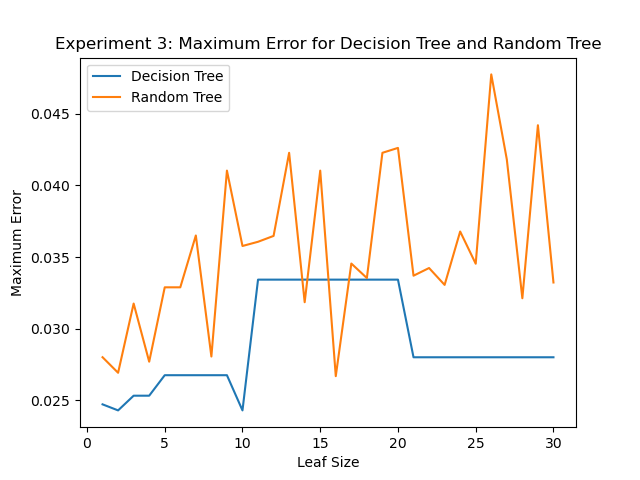
\includegraphics[height=6cm]{Figures/Figure3.png}%
\captionof{figure}{This figure shows the Maximum Error from a Decision Tree and Random Tree trained on leaf sizes ranging from 1 and 30.}\label{fig:flowchart}%
\end{jdffigure}
First, we will use the Maximum Error (ME) to measure the performance of both models.
\textbf{Figure 3} shows that w,hile the Decision Tree has a consistently lower ME, there are some leaf sizes (around 13-16) where the Random Tree performed better.
The Decision Tree also shows less variance in performance across different leaf sizes than the Random Tree.
It is reasonable to expect the Decision Tree to perform better because it makes more data-informed decisions by calculating correlations where the Random Tree makes random choices.
The data does show that in this case, the Decision Tree is likely improved enough to be worth the extra computational cost.
It is worth noting that the benefit of measuring models based solely on ME is very limited.
This is because it only shows the worst case scenario of the results, and doesn't provide any represenation of how the model performs for all other cases.

Next, we look at the time it took to train the models.
This could also be looked at as the computational cost of building the models.
While these models are small enough to be built on a personal laptop, computational cost must be considered for larger enterprise models.
We expect the Decision Tree to take longer to train because it has to calculate the best split at each node.
Meanwhile, the Random Tree has the benefit of simply choosing a split and moving on.
We'd also expect both models to take longer to train as the leaf sizes decreases, because the models have to build more leaves and perform more computations.
\begin{jdffigure}
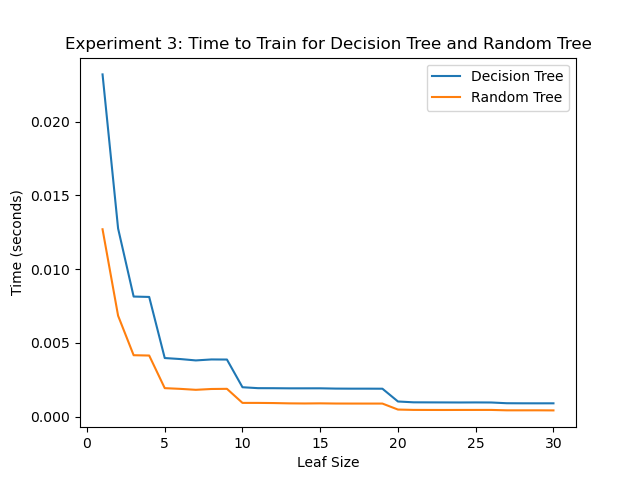
\includegraphics[height=6cm]{Figures/Figure4.png}%
\captionof{figure}{This figure shows the Time it took to train a Decision Tree and Random Tree trained on leaf sizes ranging from 1 and 30.}\label{fig:flowchart}%
\end{jdffigure}
\textbf{Figure 4} confirms our hypotheses by showing that models with smaller leaf sizes took longer to train.
Additioanlly, the Decision Tree took longer to train than the Random Tree for all leaf sizes.

In Experiment 3, we see that the Decision Tree Learner is more performant based on it's Maximum Error.
The data suggests that it will give us better results, although it is worth noting the limitations of the ME metric.
On the other hand, we see that the Time to train the Decision Tree is longer, effectively making this model more expensive.
This represents a tradeoff that we can expect to find when comparing machine learning models.
At the end of the day, the best model for a job will depend on the specific use cases and constraints.

\section{Summary}
In these experiments, we used a few different models to explore some of the tradeoffs that come with building machine learning models.
We first looked at overfitting and how different leaf sizes can impact it's effect on a Decision Tree.
We also explored how bagging techniques can help mitigate this impact and increase performance.
Finally, we compared the performance of a Decision Tree to a Random Tree and explored the tradeoffs between performance and cost.
While we found the Decision Tree to be more performant (at least based on Maximum Error), it is also more expensive to train.
Overall, we can see that there are many tradeoffs that msut be considered when building machine learning models.
Problems such as overfitting and cost mean that models cannot always be improved by simply training longer.
However, by analyzing results of test data, we can make informed decisions to cobat overfitting and optimize our models based on the metrics we deem to be most important.

\end{document}
